\begin{recipe}{Banana Muffins}{12 Portions}{30 Minutes}

Preheat oven to 350\degrees F.\\

\ingredient[1~\fr{3}{4}]{Cup}{Flour}
\ingredient[1]{Tsp}{Baking Soda}
\ingredient[\fr{1}{2}]{Tsp}{Salt}
\ingredient[1]{Tsp}{Cinnamon}
Mix dry ingredients in medium mixing bowl.\\~\\~\\~\\

\ingredient[\fr{1}{2}]{Cup}{Oil}
\ingredient[\fr{1}{3}]{Cup}{Yogurt/Milk}
\ingredient[1]{Tsp}{Vanilla Extract}
\ingredient[3]{}{Bananas}
\ingredient[2]{}{Eggs}
Mix wet ingredients in large mixing bowl.\\~\\~\\~\\~\\

\newstep
Add dry ingredients to wet mixture and mix well.\\

\newstep
Grease 12-cup muffin pan and add mixture.\\

\ingredient[]{Optional}{Nuts}
\ingredient[]{Optional}{Seeds}
\ingredient[]{Optional}{Chocolate Chips}
Optionally top muffins.\\~\\~\\

\newstep
Bake 20--22 minutes, until fork comes out clean.

\end{recipe}

\begin{center}
~\\~\\
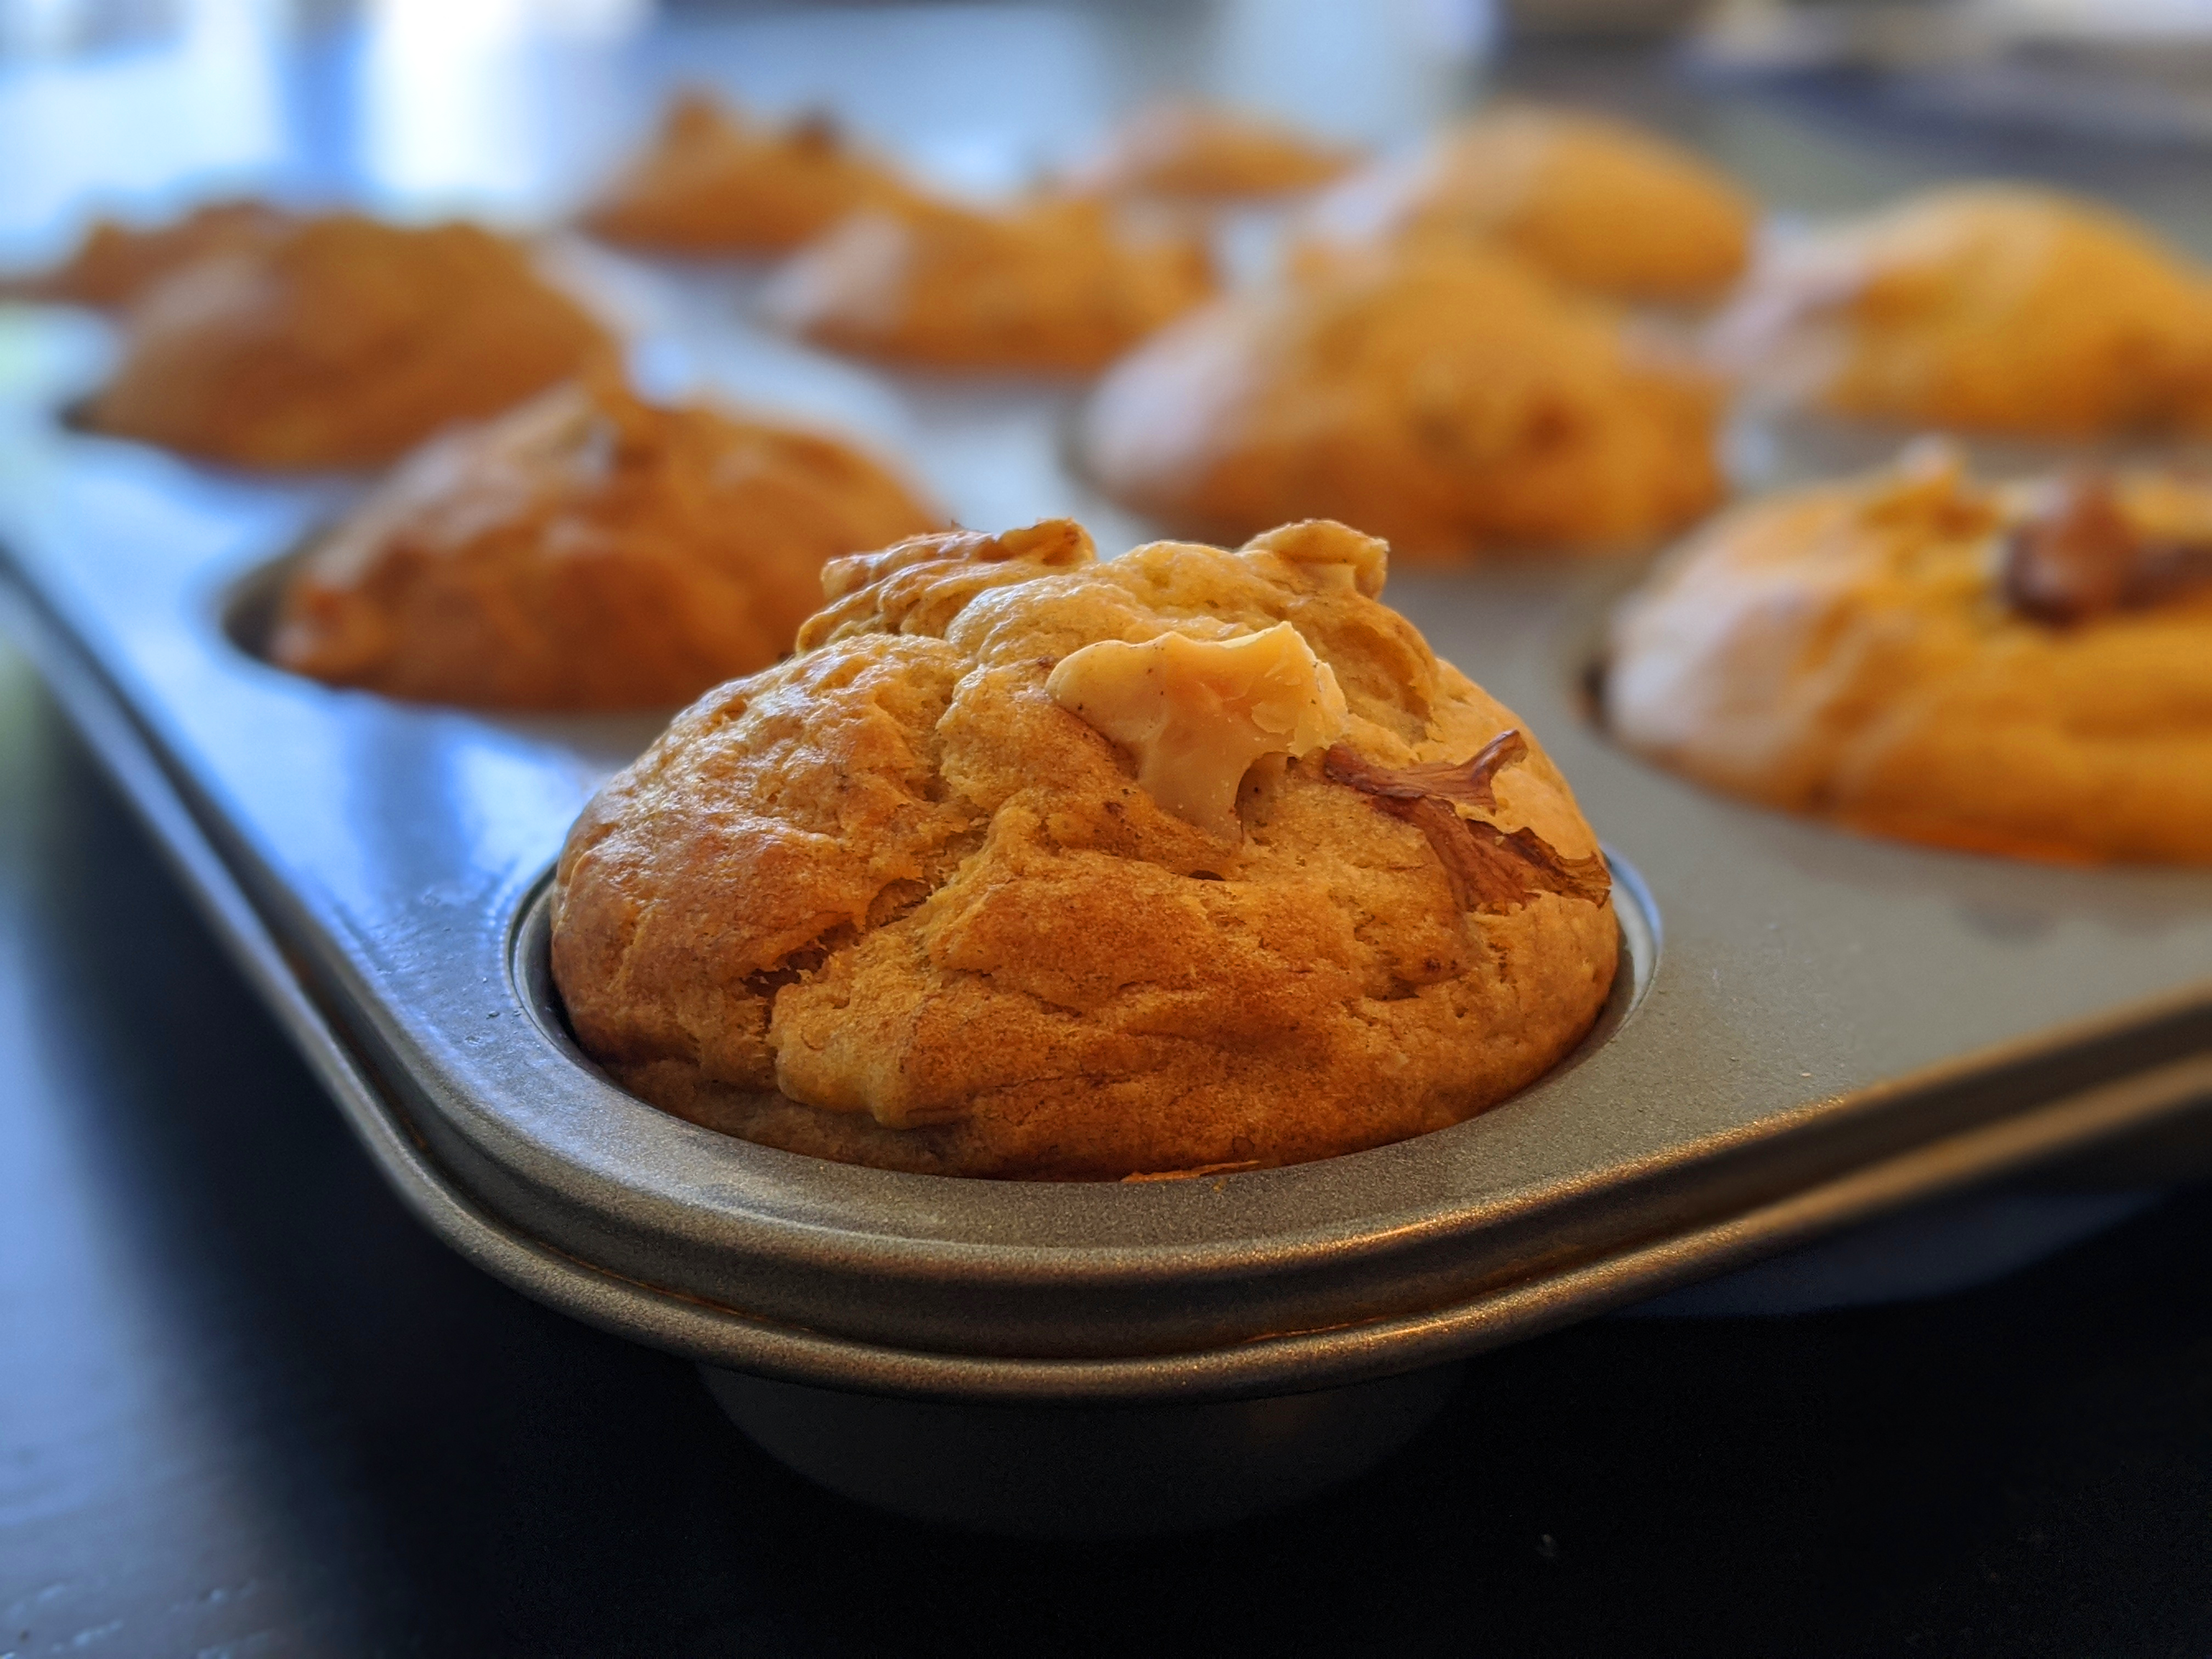
\includegraphics[width=3.5in]{baking/banana_muffins.jpg}
\end{center}